\documentclass[12pt, a4paper, oneside]{ctexart}
\usepackage{amsmath, amsthm, amssymb, bm, color, framed, graphicx, hyperref, mathrsfs, float, caption,subfigure}
\usepackage[justification=centering]{caption}

% multi-column
\usepackage{tasks}
% itemize
\NewTasksEnvironment[label=(\arabic*), label-width=3ex]{exercise}

\everymath{\displaystyle}

\title{\textbf{第九次作业\&第十次作业}}
\author{U08M11002 Spring 2022}
\date{提交截止日期:北京时间2022年6月24日}
\linespread{1}
\definecolor{shadecolor}{RGB}{241, 241, 255}

\newcounter{problemname}
\newenvironment{problem}{\stepcounter{problemname}\par\noindent\textbf{题目\arabic{problemname}. }}{\\\par}
\newenvironment{warning}{\begin{shaded}\par\noindent\textbf{提交作业方式:}}{\end{shaded}\par}

\begin{document}
	
	\maketitle	
	
	\begin{warning}
		具体提交方式请以 QQ 群里助教的通知为准。
		\begin{enumerate}
			\item 为了你自己复习需要,\textbf{建议上交前自行扫描备份}。
		\end{enumerate}
	\end{warning}
	
	\hspace{1em}
	
	
	\begin{problem}
		已知两个系统函数$H(s)$的零极点分布如图1和图2所示,且已知$H_0 = 1$,求$H(s)$。
		\begin{figure}[H]
			
\includegraphics[width=8cm]{assets/hw910img1.png}
			\centering
			\caption{}
		\end{figure}
	\begin{figure}[H]
		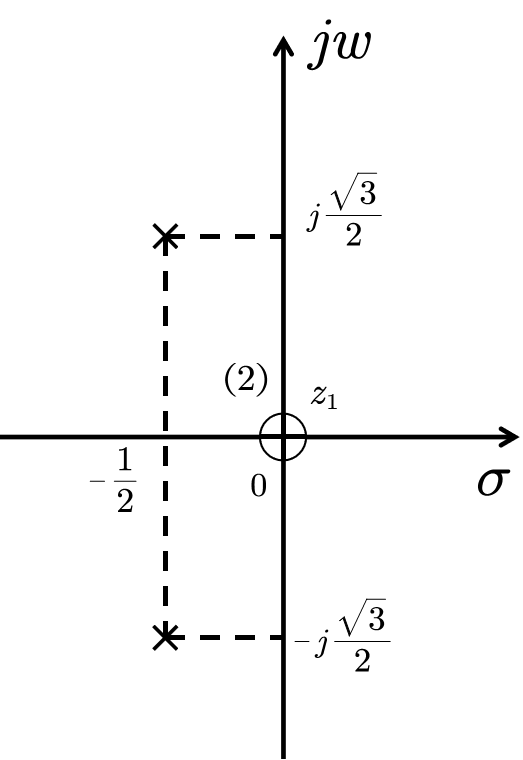
\includegraphics[width=7cm]{assets/hw910img2.png}
		\centering
		\caption{}
	\end{figure}
		\quad
	\end{problem}
	

	\begin{problem}
		已知系统函数$H(s) = \frac{s + 5}{s^{2} + 5s + 6}$;
		\begin{exercise}
			\task 写出描述系统响应$y(t)$与激励$f(t)$关系的微分方程;
			\task 画出系统的一种时域模拟图;当激励$f(t) = \delta(t)$时,求系统的全响应$y(t)$;
			\task 若系统的初始状态为$y(0^{-}) = 2$,$y^{'}(0^{-}) = 1$,激励$f(t) = e^{-t}U(t)$,求系统的零状态响应$y_f(t)$,零输入响应$y_x(t)$,全响应$y(t)$。
		\end{exercise}
		\quad
	\end{problem}
	
	\begin{problem}
		已知系统的微分方程为$y^{'''}(t) + 5y^{''}(t) + 8y^{'}(t) + 4y(t) = f^{'}(t) + 3f(t)$;
		\begin{exercise}
			\task 求系统函数;
			\task 画出系统三种形式的信号流图。
		\end{exercise}
		\quad
	\end{problem}
	
	
	\begin{problem}
		描述某$\mathrm{LTI}$系统的差分方程为$y(k) - y(k-1) -2y(k-2) = f(k) + 2f(k-2)$,已知$y(0) = 2$,$y(1) = 7$,激励为$f(k) = U(k)$。用$z$变换法求系统的零输入响应、零状态响应和全响应。
		\quad
	\end{problem}
	

	\begin{problem}
		某线性时不变因果系统,当初始状态为$y(-1) = 0$,$y(-2) = 0.5$,激励为$f(k) = U(k)$时,系统全响应为$y(k) = [1 - (-1)^{k} - (-2)^{k}]U(k)$。求差分方程。
		
		\quad
	\end{problem}
	
	\begin{problem}
		已知某$\mathrm{LTI}$因果系统的差分方程为:$y(k) + 0.2y(k - 1) - 0.24y(k - 2) = f(k) + f(k - 1)$
		\begin{exercise}
			\task 求系统函数,并指明收敛域;
			\task 画出级联形式的信号流图;
			\task 判断系统的稳定性;
			\task 若激励为$f(k) = 2\cos(0.5\pi k + 45^{\circ})$,求正弦稳态响应。
		\end{exercise}
		\quad
	\end{problem}
	
	\begin{problem}
		已知某$\mathrm{LTI}$因果系统模拟图如图3所示。
		\newline
		当激励为:	$f(k) = 1 + 2\cos(0.5\pi k) + 3\cos(\pi k)$
		\newline
		求稳态响应。
		\begin{figure}[H]
			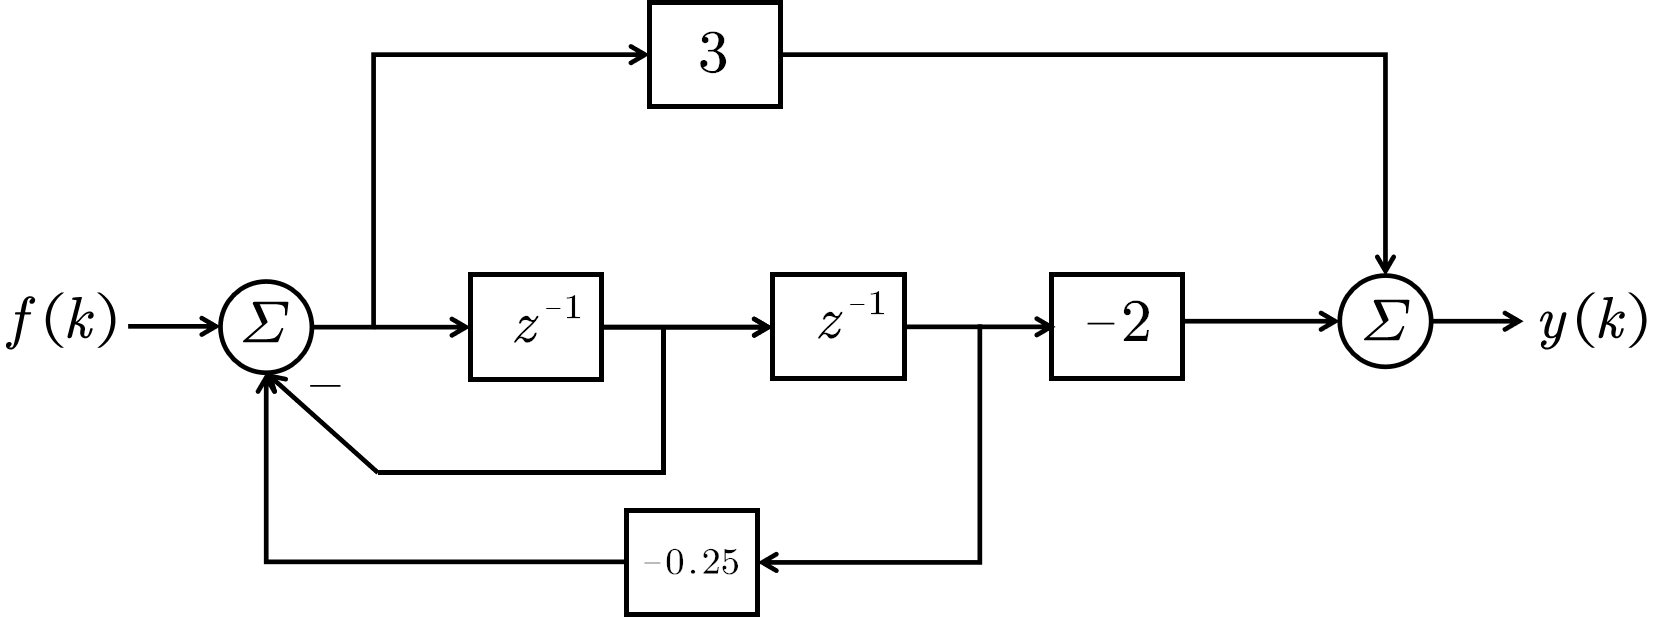
\includegraphics[width=10cm]{assets/hw910img3.png}
			\centering
			\caption{}
		\end{figure}
		\quad
	\end{problem}
	
	\newpage
	\begin{problem}
		已知离散系统的差分方程为$y(k) - y(k -1) - 2y(k - 2) = f(k) + 2f(k - 2)$,系统的初始状态为$y(-1) = 2$,$y(-2) = -\frac{1}{2}$;激励$f(k) = U(k)$。求系统的零输入响应$y_x(k)$,零状态响应$y_f(k)$,全响应$y(k)$。
		\quad
	\end{problem}
	
	\begin{problem}
		已知离散系统的差分方程为$y(k) - \frac{1}{3}y(k - 1) = f(k)$。
		\begin{exercise}
			\task 画出系统的一种信号流图。
			\task 若系统的零状态响应为$y_f(k) = 3[(\frac{1}{2})^{k} - (\frac{1}{3})^{k}]U(k)$,求输入$f(k)$。
		\end{exercise}
		\quad
	\end{problem}
	
	\begin{problem}
		已知离散系统的信号流图如图4所示。
		\begin{exercise}
			\task 求$H(z) = \frac{Y(z)}{F(z)}$及单位序列响应$h(k)$;
			\task 试判断系统的稳定性;
			\task 写出系统的差分方程;
			\task 求系统的单位阶跃响应$g(k)$。
		\end{exercise}
	\begin{figure}[H]
		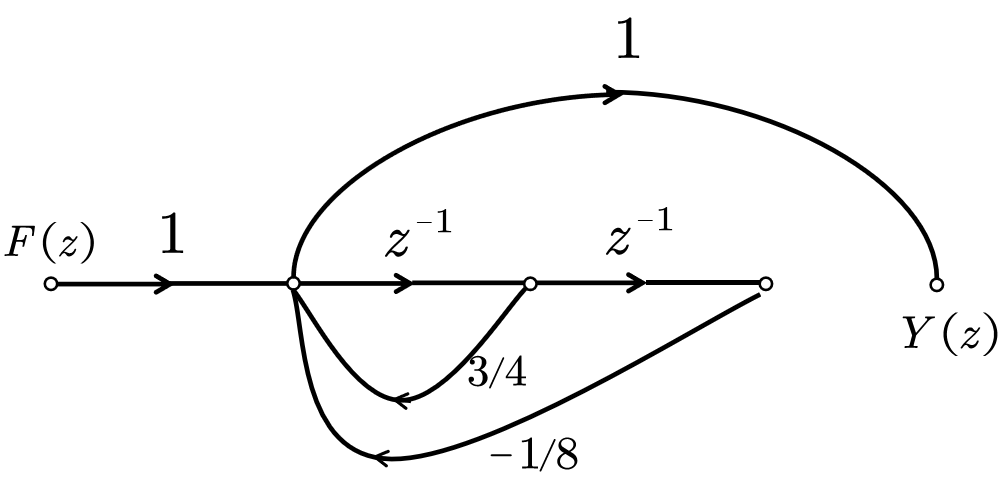
\includegraphics[width=10cm]{assets/hw910img4.png}
		\centering
		\caption{}
	\end{figure}
		\quad
	\end{problem}

\newpage
	\begin{problem}
		已知系统的状态方程与输出方程为
		\begin{equation}
			\left[
			\begin{array}{cccc}
				\dot{x_1(t)}\\
				\dot{x_2(t)}
			\end{array}
			\right ]
			=
			\left[
			\begin{array}{cccc}
				-2&1\\
				0&-1
			\end{array}
			\right ]
			\left[
			\begin{array}{cccc}
				x_1(t)\\
				x_2(t)
			\end{array}
			\right ]
			+
			\left[
			\begin{array}{cccc}
				1\\
				0
			\end{array}
			\right]f(t)
		\end{equation}
	\begin{equation}
		y(t)
		=
		\left[
		\begin{array}{cccc}
			1&0
		\end{array}
		\right ]
		\left[
			\begin{array}{cccc}
				x_1(t)\\
				x_2(t)
			\end{array}
		\right]
	\end{equation}
		初始状态
		\begin{equation}
			\left[
			\begin{array}{cccc}
				x_1(0^{-})\\
				x_2(0^{-})
			\end{array}
			\right]
			=
			\left[
			\begin{array}{cccc}
				1\\
				1
			\end{array}
			\right]
		\end{equation}
		激励$f(t) = U(t)$。求状态向量$x(t)$,响应$y(t)$,转移函数$H(s)$,冲激响应$h(t)$。
		\quad
	\end{problem}

	\begin{problem}
		已知离散系统的状态方程与输出方程为
		\begin{equation}
			\left[
			\begin{array}{cccc}
				x_1(k+1)\\
				x_2(k+1)
			\end{array}
			\right]
			=
			\left[
			\begin{array}{cccc}
				\frac{1}{2}&\frac{1}{4}\\
				1&\frac{1}{2}
			\end{array}
			\right]
			\left[
			\begin{array}{cccc}
				x_1(k)\\
				x_2(k)
			\end{array}
			\right]
			+
			\left[
			\begin{array}{cccc}
				1\\
				0
			\end{array}
			\right]
			f(k)
		\end{equation}
	
	\begin{equation}
		\left[
		\begin{array}{cccc}
			y_1(k)\\
			y_2(k)
		\end{array}
		\right]
		=
		\left[
			\begin{array}{cccc}
				1&0\\
				0&1
			\end{array}
		\right]
		\left[
		\begin{array}{cccc}
			x_1(k)\\
			x_2(k)
		\end{array}
		\right]
		+
		\left[
		\begin{array}{cccc}
			1\\
			1
		\end{array}
		\right]
		f(k)
	\end{equation}
		初始状态为
		\begin{equation}
			\left[
			\begin{array}{cccc}
				x_1(0)\\
				x_2(0)
			\end{array}
			\right]
			=
			\left[
			\begin{array}{cccc}
				1\\
				1
			\end{array}
			\right]
		\end{equation}
		激励$f(k) = U(k)$。用$z$变换法求:
		\begin{exercise}
			\task 状态转移矩阵$\Lambda^{k}$;
			\task 状态向量$x(k)$;
			\task 响应向量$y(k)$;
			\task 转移函数矩阵$H(z)$;
			\task 单位响应矩阵$h(k)$。
		\end{exercise}
		\quad
	\end{problem}


\end{document}